\documentclass{article}
\usepackage[utf8]{inputenc}
\usepackage{caption}
\usepackage{graphicx}
\usepackage{subfigure}
\usepackage{geometry}
\geometry{a4paper,scale=0.83}

\title{ARM11 Assembler and Emulator}
\author{Taowen Liu, Sihan Tao, Chuxuan Li, Ranchen Li}
\date{June 2021}

\begin{document}

\maketitle

\section{Introduction}
In this project, we worked with a family of Reduced Instruction Set Computer-based (RISC) computer processors.
We implemented an ARM emulator, which simulates the execution of an ARM binary file, and an ARM assembler, which translates an ARM assembly source file into a binary file that the emulator can subsequently execute. Our emulator and assembler support a subset of the ARM instruction set, including 
the Data Processing, Multiply, Single Data Transfer, and Branch instructions.

\section{Implementation}
\begin{itemize}
    \item \textbf{src} contains three directories: \textbf{global\_utils}, \textbf{emulator} and \textbf{assembler}.
    \item \textbf{global\_utils} contains the type definitions, helper functions and a simple test suite used in both assembler and emulator.
    \item \textbf{emulator} contains all the source files of the emulator.
    \item \textbf{assembler} contains all the files needed to implement the functionality of the assembler.


\end{itemize}



\begin{figure}[ht]

\begin{minipage}{0.6\linewidth}
    \subsection{Global\_utils}
    \textbf{Global\_utils} is structured as follow:
    \begin{itemize}
        \item \texttt{tools.[ch]} contains four functions used for bit operations, which are called frequently in both assembler and emulator.
        \item \texttt{type\_and\_macros.h} includes the definition of all the macros, enumerators and structures. These enums and macros significantly increase the readability and maintainability of the code, avoiding magic numbers. The structures are defined hierarchically, which means larger data types consist of smaller components, simplifying the sophisticated logic. In addition,  unions are used to save space.
        \item \texttt{unit\_test.[ch]} is a simple test suite, supporting the equality test of int, double, long, char, float, boolean value and string.
    \end{itemize}
    
    \subsection{Emulator Implementation}
    	We have created the following: Main, Decode, Execute, Utils and Tests. The Main module depends on the Execute and Decode module. Furthermore, the Utils module is essential for all other modules as data types and common helpers are defined there. Please see the Figure \ref{fig:Emulator dependency graph} below for the emulator dependency graph.
\end{minipage}
\quad
\begin{minipage}{0.5\linewidth}
    \centering          
    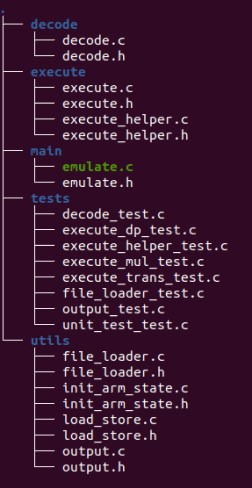
\includegraphics[width=0.55\hsize]{./final_report_figure/tree_emulator} 
    \caption{Emulator tree} 
\end{minipage}
\end{figure}

\begin{figure}
    \centering
    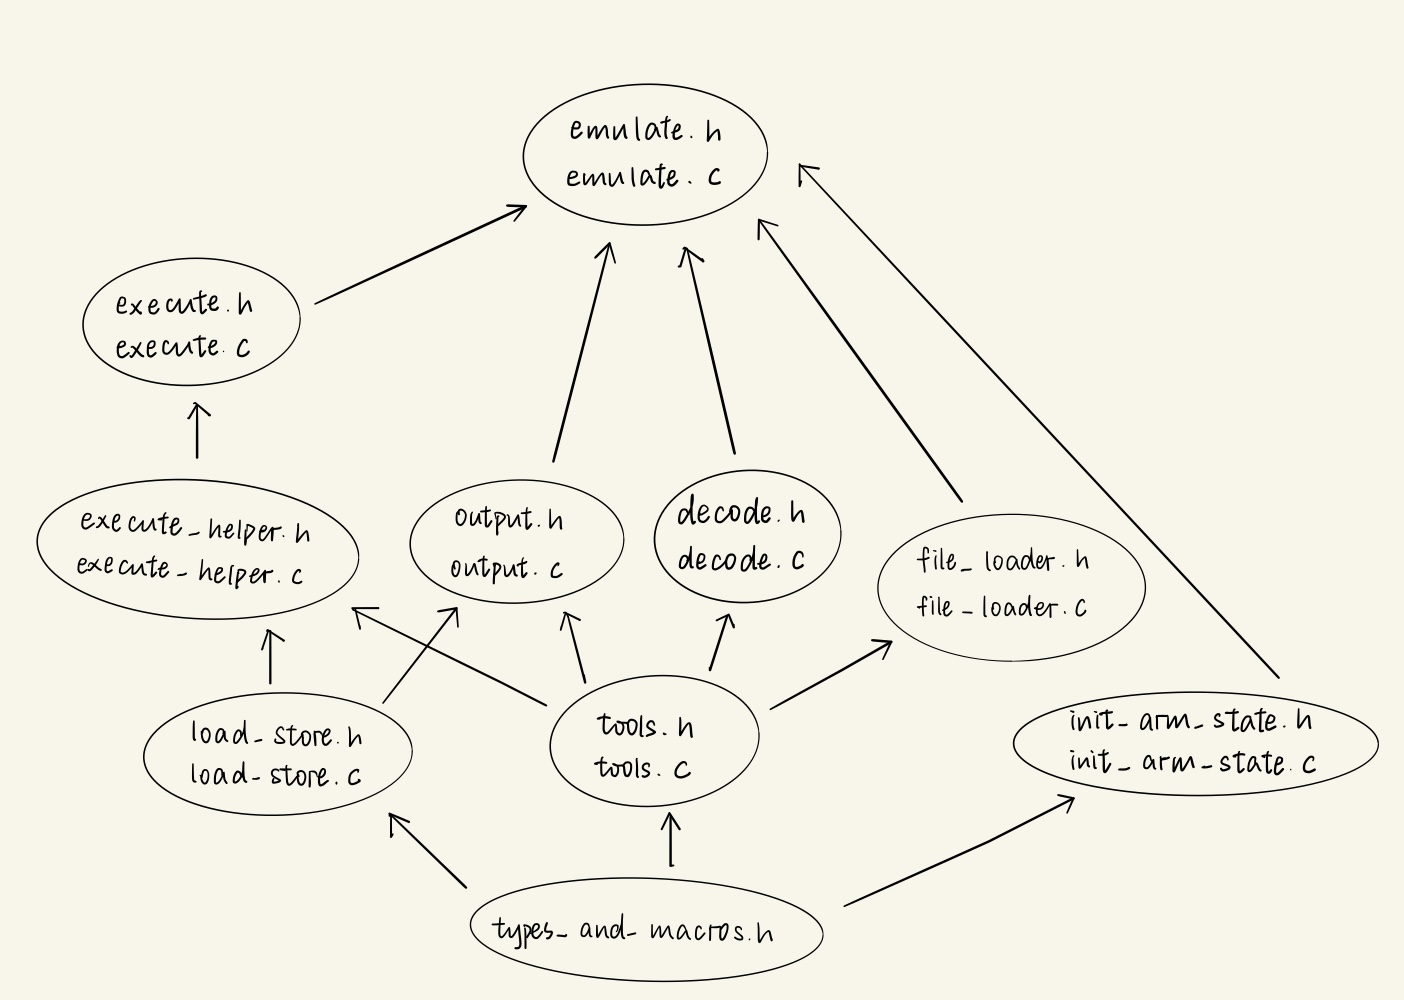
\includegraphics[width=0.4\hsize]{./final_report_figure/emulator_dependency_graph}
    \caption{Emulator dependency graph}
    \label{fig:Emulator dependency graph}
\end{figure}

\begin{itemize}
    \item \textbf{Main module} contains \texttt{emulate.c} and its header file. \texttt{emulate.c} is the entry point of the emulator program. It takes a single filename as an argument that contains the ARM11 object code. Then it calls \texttt{init\_memory} from \texttt{file\_loader.h} to load the file into memory, followed by \texttt{init\_pipelines}, \texttt{preheat\_pipeline} to create the fetch-decode-execute pipeline. After that, \texttt{decode} and \texttt{execute} from \texttt{decode.h} and \texttt{execute.h} is called respectively for the three-stage pipeline. Finally, before main frees all the allocated memory on the heap, it calls \texttt{output} from \texttt{output.h}, which prints the registers and non-zeroed memory in the automated test format. 
    
    \item \textbf{Decode module} contains \texttt{decode.c} and its header. \texttt{decode.c} accepts a fetched instruction of unknown type as an argument and returns the intermediate representation defined in \texttt{types\_and\_macros.h} in \texttt{global\_utils}.
    
    \item \textbf{Execute module} \\
    \texttt{execute.c} contains the dispatcher, which calls the sub-functions according to the instruction tag. Specialized functions are written to deal with the four kinds of instructions in \texttt{execute\_helpers.c} where we also integrated some helper functions(data rotation ...) used in the execution module.
    
    \item \textbf{Utils module} \\
    \texttt{file\_loader.c} load the ARM object code in the memory structure we defined. \texttt{init\_arm\_state.c} initialize the state of the arm machine. \texttt{load\_store.c} allows us to load or store information from(to) the
    memory of the ARM machine. \texttt{output.c} prints out the registers and non-zeroed memory, which satisfies the given automated test suite format.
    \end{itemize}

\subsection{Assembler Implementation}
We have created the following Directories: Main, Data Structure, and Combinators. Instead of creating the parser and encoder top-down, we first made small and essential components of the parser and encoder and integrated them into larger components. Please see the Figure \ref{fig:Assembler dependency graph} below for the emulator dependency graph.

\begin{figure}
    \centering
    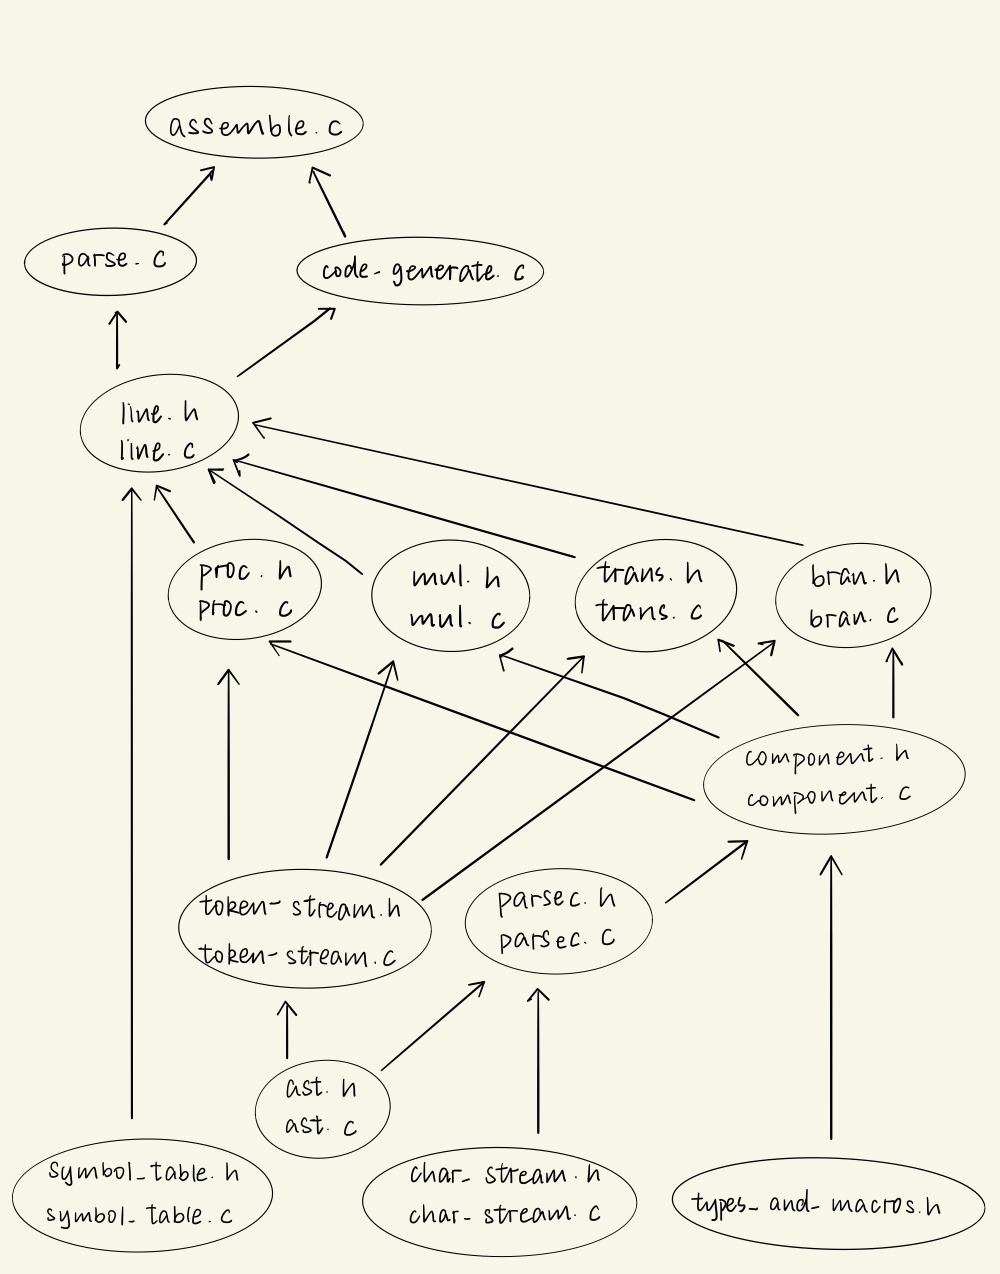
\includegraphics[width=0.4\hsize]{./final_report_figure/assembler_dependency_graph}
    \caption{Assembler dependency graph}
    \label{fig:Assembler dependency graph}
\end{figure}

\begin{itemize}
    \item \textbf{Main module} contains \texttt{assemble.c}, \texttt{code\_generate.c} and \texttt{parser.c}. We implemented a two-pass assembler in \texttt{assemble.c}. 
    The first pass parses the input files, converting instructions to \textit{abstract syntax tree (AST)} defined in extension parsec and associating symbols with their memory addresses through symbol table. 
    The second pass generates corresponding binary code by calling functions in \texttt{code\_generate.c}. This \texttt{.c} file first converts \textit{AST}s into an intermediate representation of instruction, which is further converted into required binary code.
    \item \textbf{Data Structure module} contains \texttt{symbol\_table.c} and \texttt{token\_stream.c}.\\
    \textbf{symbol\_table.c} defines the symbol table as a binary tree, mapping labels to addresses. One advantage of the binary tree implementation is its simplicity and efficiency over the linked list implementation. \texttt{add\_node} is used to edit the table, and \texttt{find\_node} gives us the required address. In addition, \texttt{free\_node} is called to free allocated memory, avoiding memory leaks.\\
    \textbf{token\_stream.c} defines \texttt{token\_t} and \texttt{token\_stream\_t} structures. A token represents a line of the assembly code, and a token stream is a linked-list-based queue. It provides interfaces \texttt{init\_token\_stream}, \texttt{add\_token\_stream}, \texttt{pop\_token\_stream,} \texttt{free\_token}, and \texttt{free\_token\_stream} functions to initialize the token stream, add and pop the token element to or out the given stream, and free all allocated memory.
    \item \textbf{Combinators module} contains the logic for parsing and code generating.
    Enabled by our extension parser combinator, we built our parser and code generator bottom up. 
    We first constructed component parser combinators. Then we build larger parser combinators based on those smaller ones.
    Using these small parser combinators, we finally built parser combinators for instructions and the whole line.
\end{itemize}

\section{Testing}
\subsection{Structure of Testing}
\begin{itemize}
    \item \textbf{unit test} \\
    We adopted test-driven development(TDD) for our project. An individual test was designed for each function, enhancing debugging and developing efficiency. This means we could test the file once it is completed due to low dependency between files. Besides, writing new functions or files based on tested ones could be pretty straightforward. 
    \\For example, when writing the parser and code generator, we could test the correctness of our parser while building them.
    The workflow is: write a parser combinator, write the code generator for that parser, and write a test to check the pair. If the parser correctly parses a string, the code generator correctly encodes to produce an intermediate representation.

    \item \textbf{Python script} \\
    There are so many unit test files that it would be tedious to test them by hand. Hence we designed a python script called testall to enable the automated testing of all the unit tests. To use it, simply type in \texttt{make test} in the \textbf{arm11\_49} directory.
    \item \textbf{Ruby test suite} \\
    The test suite was handy as it gave us an idea of whether our emulator and assembler were working or not. We tested our project with the it until we passed all the unit tests. If some cases failed, we could go back to add cases in unit tests and locate the bugs quickly.
\end{itemize}
\subsection{Advantages of unit test design in practice}
In one of the assembler tests, we did not expect that a negative hexadecimal number would appear. Thanks for the design of \texttt{parsec} and unit tests, we only need to modify the function \texttt{p\_hexa} in order to check it is negative or not.
Besides, we missed the case where brackets at the front of a register at first, but similarly, it was solved by add match cases in \texttt{p\_reg\_i}.
Another example is that we did not realize that the label contained a number (such as wait1:) until we ran the Ruby test suite. And we fixed it quickly due to the unit test.
\subsection{A Failed Test}
Although our design of the parser combinator is creative, a small mistake occurred when testing the assembly line \texttt{str r1,[r2],r4}. that was because our parser used the greedy match algorithm, and we did not have enough time to fix logic in it. 
\section{Extension: Parsec}
\textbf{Parsec(Parser combinator)} is a library to build parsers using the C programming language, inspired by a Haskell library with the same name.
It allows us to build a parser from the bottom up so that a larger parser can be composed of smaller ones. This means parsers built in this way are reusable and testable. Besides, correct use of parser combinator can save the user from the trouble of memory management.

\subsection{Usage}
All parser combinators consist of atomic parser combinators. For example, a register parser combinator (r1) contains a single character parser ‘r’ followed by a number parser combinator, which are both atomical parser combinators. Then larger ones can be built from smaller components. Finally, by combining these components, users can write a parser combinator for a piece of instruction, a line, or even a file.\\
Parser combinator enables the \textit{Read, Eval, Print and Loop (REPL)} parsing, where users first write a parser, then the user writes an AST converter for that parser, which converts the AST to a C data structure. Then the user writes a test for the parser AST converter pair before modifying the parser and AST converter accordingly.
Finally, larger parsers are built from the tested ones to guarantee correctness.
\subsection{Modularity}
\textbf{Parser combinator} consists of 3 modules.
The implementation of each module is independent of the other two so that the user can choose to use any number of these modules.
Also, the user can provide their own implementation, as long as the implementation fits the format in the interfaces.
\begin{itemize}
    \item \textbf{ast.[ch]} \textit{(abstract syntax tree)} provides the data structure for the result of parsing, which is implemented as a string to string tree map since the C programming language does not provide subclass polymorphism.
    \item \textbf{char\_stream.[ch]} provides the data structure for the input of parsing. It is essentially a sequence of char that allows trace back operation.
    \item \textbf{parsec.[ch]} provides atomic parser combinator constructors and a main function called \texttt{perform parse}, which takes a parser combinator and a char stream as an input and outputs an AST. Interestingly, the \texttt{map\_while\_build} parameter is a newly added experimental feature, which allows the user to modify the abstract tree while building it.
\end{itemize}

\subsection{Extendibility of Parsec}
Although we only provided a minimum implementation, extending the functionality of the parser combinator is surprisingly straightforward. For example, the minimum implementation does not support the \texttt{take while} operation. To enable this operation, the user only needs to provide an atomic parser combinator constructor, a parser combinator performer, before finally register this operation to the dispatcher.

Parsec is greedy, left associative and supporting trace back operation. The matching logic of Parsec is similar to regular expression. Sequence of defining combinators is essential in Parsec, but the behaviour of Parsec is predictable. Testing while building parsers can saves users from errors.

\section{Quality Assurance}
\subsection{Code Style}
    \begin{itemize}
        \item \textbf{clang formatter}
        We installed the clang formatter and used the same configuration file to maintain the consistency of the code style and kept the function names meaningful, making the program easier to understand. 
         \item \textbf{Doxygen-style comments}
        Doxygen-style comments are added above every function to keep the project documented to ensure the readability and maintainability of our project.
        \item \textbf{Private function and naming space}
         We put helper functions in separate files or as static functions to simulate private functions which makes the main function concise. Hence namespace problems are resolved and debugging becomes simpler. 
    \end{itemize}

\subsection{Code Review by other members}
    After each file or complicated function is completed, the person who wrote the code would explain to other members what has been done and through Teams. Then others would give their suggestions on implementation and code style.      



\section{Group Reflection}
    We started our project by determining the structure, splitting the project into modules, and defining some critical data types. Then tasks were assigned to each member according to modules and functions. The modularity of our codes enables us to clarify work distribution, improved readability and assigned tasks rapidly.\\
    We did an excellent job on collaboration and used several apps to keep track of the project.  We supervised the progress of each member on Trello, used Wechat as a resource-sharing platform, and communicated through Teams frequently. During the COVID 19 pandemic, when face-to-face communication was impossible, we communicated through video calls to allocate tasks, exchange ideas, program in pairs, and explain written codes to others. This ensured that every group member comprehends the progress of the project and can finish the tasks efficiently. In the next project, we will further utilize the functions provided by those apps to assist the project development. \\
    We use git for version control in our project. First, we created a branch for each group member, where a member worked on his/her tasks on the specific branch. However, later we accepted the advice from our mentor and switched to feature-oriented development. Branches were created for independent functions and everyone could work on them. solving the merge conflicts problems. We will apply the convention in the next project. \\
    In addition, we have created shared Google Docs for collaborating on the video presentation, and a shared Overleaf project for the final report. Shared docs are convenient for us to work together and give advice to each other.\\
    Overall, our group worked well together. We will maintain the good conventions next time since they stimulate group organization and communication, increasing the efficiency of programming and debugging.\\
    We also had some problems to avoid next time. We need to improve our time management ability because some members failed to meet the internal deadline due to unexpected difficulty in programming. It delayed our progress, and we tried to finish the project in a hurry in the end. 
\section{Individual Reflection}
\begin{itemize}
    \item \textbf{Taowen Liu}\\
    Our group collaborated well. Teams call and pair programming is something we used frequently in our project. They are incredibly helpful for debugging. Doing code review allows us to improve the cleanness and correctness of our codes. All group members have their own strength, which we can learn from each other.\\
    I think my strength in our group is that I am good at structural designing, familiar with C programming language and I had some prior experience in building parser and emulator. A lot of design I put forward has been proven helpful in aspect of improving readability and maintainability. Helping others through teams call made me feeling proud and being needed.\\
    I learnt some new git operation through this project, which I felt rewarding. From the lectures and extracurricular reading
    , I learned a lot of conventions and skills in C programming, which they were useful in our project. Through this project, I gained some experience in how to present my work which will be important in future career. Using gdb to debug is also another useful skill I learnt in this project.\\
    Through implementing our extension parser combinator, I gained new understanding toward data structure and how to create dynamic structures in less flexible language.\\
    Leadership skill is one aspect that I can improve on. In this project, I tend to assign too much work on myself. In the next project, I will put more effort on motivating group members and distributing work according to their ability, which this skill would be helpful in future career.\\
    Another aspect I can improve on is that I can improve my communication skill. Sometimes I find its would cost to much time to explain new concepts to my group member, so that I chose to implement them on myself.\\
    \item \textbf{Sihan Tao}\\
    I am well integrated with the group and made a significant contribution to the project.\\ 
	One of my strengths is my programming skills and clean code style. I played an important role in deciding the project structure and defining the essential data types. Some data types and structures I defined are used throughout the whole project. I also wrote many helper functions in advance used by other teammates. Moreover, I advised on documenting our functions and wrote half of the comments in the Doxygen format. Macros are defined to avoid magic numbers. My work contributes to increasing the readability and maintainability of our code. However, I sometimes got stuck when implementing some functions, so I will spend more time on programming in the future.\\
	Another strength is that I am self-motivated and willing to learn new skills. I have not known much of C before, but I spent much time reading books and writing codes to learn more features of C. This proves to be very useful as I learned some good conventions and features not covered in lectures in the books, applying them in the project. In addition, I learned the basics of Makefile and how to use tools to build makefiles automatically, which helps build our unit test. Next, I gain experience in git version control, and I think now I am pretty familiar with git. Last but not least, I learned how to write a LaTeX report. Although I have no experience with LaTeX before, I completed the final report.\\
	In addition, I am good at teamwork. I set up the Trello board to track the progress of group members. Besides, I pushed our group to meet more frequently on Teams and suggest using Google Docs to work together. \\
	Surprisingly, my English writing skills made a significant contribution to the final report and the video presentation. I wrote the final report and the presentation script based on their drafts, enriching the sentence patterns and making the text more coherent. \\
	In the future, I will spend more time on programming since I sometimes got stuck when implementing some functionalities. \\
	Overall I fitted well in the group and enjoyed solving problems together. I have improved my programming skills and coordination skills. In addition, I have gained experience in git, Makefile, and LaTeX. The group project was challenging and rewarding. I'm looking forward to the next one!
    \item \textbf{Chuxuan Li}\\
    I think our group worked well together. We used Trello to registered and supervised our progress. Also, we used Teams frequently to discuss and explain our own work to others, and debugging together through the share screen.\\ My strength in the group is to fill in the contents of the function, designed tests, and edited videos. During the teamwork, I wrote lots of tests for functions and each with different values, filled some functions that my teammates designed and wrote some report. I had a good experience with pair programming, as I had no C experience before, so I was not very familiar with it, but my teammates help me a lot during pair programming. Sometimes I got stack in writing the function and debugging, and I asked help for my teammates. They would help me to solve my problem or give me some ideas and explain them to me. In the next time, I will try to write more functions and designed the structure. \\
    During this project, I gained the experience on how to use the git branch, which avoid the problem of merge conflict. Also, I learnt how to use latex in this project to write report as well.\\
    Overall, I think I fitted into our group well, and I really enjoyed the process of designed and implemented the project and all the teammates work hard.

    \item \textbf{Ranchen Li}\\
    I thought the cooperation in our group was wonderful. At the start of the project, we immediately planned the structure and set a todo list using Trello, each of us clocked in everyday in order to see the progress of each others work.\\
	My main strength in the group is I’m familiar with implementing algorithms. During the teamwork, I implemented lots of useful helper functions. And thanks for the pair programming method used in our group, me and my teammate can review and test each others code efficiently.\\
	Besides, the communication between group members was also incredible well. Each time we faced a problem in coding or testing, a teams chat would be immediately set up to solve it.
	My weakness in this project would be I’m not quit familiar with C and Architecture at the start, it was also hard for me to balance my time with lectures and project at first. But with the progressing of the project and helps from my team these issues were solved very soon.\\
	Overall I thought that I integrated into our group very well, all of my teammates worked really hard for the project and felt happy with the result we reach.

\end{itemize}
\end{document}
